\section{Uncertainty of parameters}

\subsection{Method}
For varying different parameters simultaneously a similar method was used as in section \ref{sec:results-yields}, where a ``fudge-factor'' was applied to the \eris\ best fitted parameter-values. The ``fudge-factor'' is distributed gaussian around 1.0 and the factor is the multiplied to the parameter-value.

%% The parameter values chosen are the ones that deal with r-process production; fraction of neutron stars that merge (number of mergers), the ejecta mass from a single neutron star merger, the delay-time distribution of merging events.
%% Also the relevant r-process isotopes \re{187}, \re{185}, \w{184}, \os{188}, and the relevant s-process isotopes \os{187}, \os{186}.
%% These are chosen because they lie close to the \re{187}-\os{187} pair in the chart of nuclides and also closely related to the s-process path (and branching path).

\subsubsection{Monte Carlo experiment}
%add code snippet and explain how omega was used after fitting
\label{sec:mod-omega2}

In order to manipulate several yield-values in \omegamodel\ at once, a modification to \verb|__set_yield_tables| in \chemevol\ were implemented.
This is similar to the modification in section \ref{sec:mod-omega}, but includes list for all isotopes and ``fudge factors'' applied.

Other input variables are multiplied with a similar factor before the \omegamodel-simulation is executed.

\begin{lstlisting}[style=custompython, caption={Some caption}]
####################################################
### End of function as written in 'chem_evol.py' ###
""" 
Change ytables(multiply yields of 'isotope' with 'factor')
This step requires 
'self.loa_manip_isotope' and 'self.loa_manip_yields'!
"""
####################################################

#AGB + massive stars, and pop3 stars
#loop over the different objects
for table_object, table_name in zip([self.ytables, self.ytables_pop3],
                                    ["agb/massive", "pop3"]):
    #get list of available metalicities
    loa_metallicities = table_object.metallicities
    for Z in loa_metallicities:
        #get list of masses for each metallicity
        loa_masses = table_object.get(Z=Z, quantity="masses")
        for M in loa_masses:
            #loop over all isotopes to manipulate
            for manip_isotope, manip_factor in zip(self.loa_manip_isotopes,self.loa_manip_yields):
                #get current yield 
                try:
                    present_yield = table_object.get(M=M, Z=Z, quantity="Yields",
                                                     specie=manip_isotope)
                except IndexError: #this means that isotope doesn't exist for this table
                    continue
                #modify yield by some factor
                new_yield = present_yield*manip_factor 
                #"insert" new yield back into table
                table_object.set(M=M, Z=Z, specie=manip_isotope, value=new_yield)
                #print "Fixed new yield(%s): from %1.4e to %1.4e"%(table_name,present_yield, new_yield)

# SN1a, NS-NS merger, BH-NS merger
#loop over different objects
for table_object, table_name in zip(
        [self.ytables_1a, self.ytables_nsmerger, self.ytables_bhnsmerger],
        ["sn1a", "nsm", "bhnsm"]):
    #get list of available metalicities
    loa_metallicities = table_object.metallicities
    #loop over metallicities
    for i_Z, Z in enumerate(loa_metallicities):
        #loop over all isotopes to manipulate
        for manip_isotope, manip_factor in zip(self.loa_manip_isotopes,self.loa_manip_yields):
            # get index of isotope
            index_iso = self.history.isotopes.index(manip_isotope)
            #get current yield
            try:
                present_yield = table_object.yields[i_Z][index_iso]
            except IndexError: #this means that isotope doesn't exist for this table
                continue
            #modify yield by some factor
            new_yield = present_yield*manip_factor
            #"insert" new yield back into table
            table_object.yields[i_Z][index_iso] = new_yield
            #print "Fixed new yield(%s): from %1.4e to %1.4e"%(table_name,present_yield, new_yield)
return
\end{lstlisting}


%explain data
\subsubsection{Postprocessing}
%explain beta decay on data -> create new data
%code snippet from beta-decay
\label{sec:mod-betadecay}
The output files for each \omegamodel-run consists of time-arrays for a multitude of measurables, e.g. the mass of \re{187} in the interstellar medium.
Postprocessing of all the datafiles must be done in order to account for the \betadecay of \re{187} to \os{187}\footnote{At the time of writing, \omegamodel does not account for \betadecay of radioactive nuclei, so this is implemented in postprocessing. The effect of \betadecay in \omegamodel is minimal as the total metallicity does not change, which again does not change the stellar yields considered.}.
This is done, for each timestep, by calculating the amount of decayed material from parent nucleus to daughter nucleus. The amount of decayed material is calculated from the timestep length and half-life of the radioactive parent nucleus, and applied to the current and all following timesteps for parent and daughter nuclei.
\comment{Add reference to section of \betadecay calculations}
The new data is then saved to file in the same format.
The function for applying the decay to parent nucleus and daughter nucleus (\re{187} and \os{187}, respectively, in our case) is found in listings \ref{lst:mod-betadecay}.

\begin{lstlisting}[style=custompython, caption={\label{lst:mod-betadecay}Snippet of code implementing \betadecay in postprocessing on data calculated by \omegamodel.}]
def apply_decay(self, time_array, parent_array, daughter_array, halflife):
    """ Apply decay from parent to daughter with 
    the corresponding time-array and nuclear halflife.
    Halflife in same units as time_array. """

    decay_constant = np.log(2)/halflife

    for i in range(len(time_array)-1):
        #calculate time
        dt = time_array[i+1] - time_array[i]
        #calculate decay
        dN = - decay_constant * parent_array[i] * dt
        #apply decay to parent forall indeces greater then i
        parent_array[i+1:] += dN
        #same for daughter, but negative decay
        daughter_array[i+1:] -= dN

    return parent_array, daughter_array
\end{lstlisting}

%explain 'extraction' to new data-files and subsequent reduction to plots

\FloatBarrier

\subsection{results}
%description of the different experiments
\newcommand\expone{\textbf{Yields}}
\newcommand\exptwo{\textbf{Yields+IMFslope}}
There are two main experiments;
\begin{description}
\item[\expone] The yields of isotopes are varied within their standard deviation \comment{Add reference to arnould table}
\item[\exptwo] The yields of isotopes are varied \textit{and} the high mass slope of the initial mass function, $\alpha$, is varied within the uncertainty found in \mycite{cote16a}, which is $\sigma_{\alpha}=8.73\%$ around the mean $\langle \alpha \rangle = 2.29$.
\end{description}

%present data
The solar system is formed from a collapse of interstellar gas. The gas is assumed to have separated from the interstellar medium at the formation of the solar system.
The formation of the solar system is estimated from meteorites to be 4.5 Gyrs ago \comment{add citation and expand on meteorite articles}
From the semianalytical model, \omegamodel, the total mass of \os{187} and \re{187} in the interstellar medium is calculated.
The fraction between the two isotopes, $f_{187} = \frac{\os{187}}{\re{187}}$, is also calculated.
The fraction between the isotopes is relevant because it can be determined from meteorites, unlike the total mass of isotopes in the \sos\ at the time of formation.
In the \eris-simulation the galactic age is 14 Gyrs, which means the solar system formed at 9.5 Gyrs.
The uncertainties of the mass of each isotope come from the uncertainty of the input parameters in each experiment, \expone\ and \exptwo.

%explain results/plots for each experiment
In figures \ref{fig:MCExperiment-nodecay} the evolution and distribution of \re{187}- and \os{187}-mass in the inter stellar medium is plotted, as well as the ratio between them. 
%explain how they differ

\FloatBarrier

%Use subfigwidth for the first two figures
\setlength{\subfigwidth}{0.45\textwidth}
%Use figwidth for the last figure
\setlength{\figwidth}{0.8\textwidth}

%add plots of Os-187, Re-187, Os-187/Re-187 for regular MCExperiment wo/decay
\begin{figure}
  \centering
  \begin{subfigure}{\subfigwidth}
    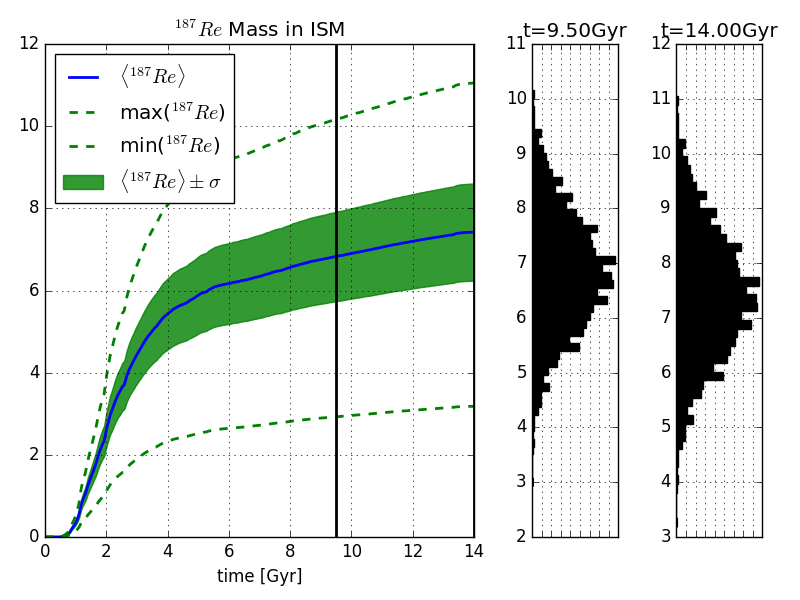
\includegraphics[width=\linewidth]{results/MCExperiment_revised_2/combined_plot_Re-187.png}
    \caption{\label{fig:MCExperiment-nodecay-re187}
      Total mass of \re{187} in the interstellar medium of the galaxy modelled by \omegamodel.
  }
  \end{subfigure}
  \begin{subfigure}{\subfigwidth}
    \centering
    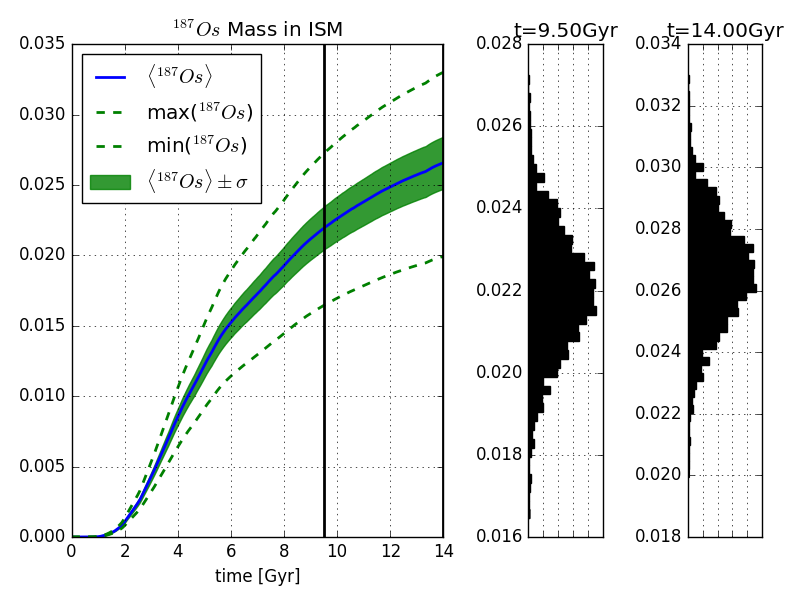
\includegraphics[width=\linewidth]{results/MCExperiment_revised_2/combined_plot_Os-187.png}
    \caption{\label{fig:MCExperiment-nodecay-os187}
      Total mass of \os{187} in the interstellar medium of the galaxy modelled by \omegamodel.
    }
  \end{subfigure}
  \begin{subfigure}{\figwidth}
    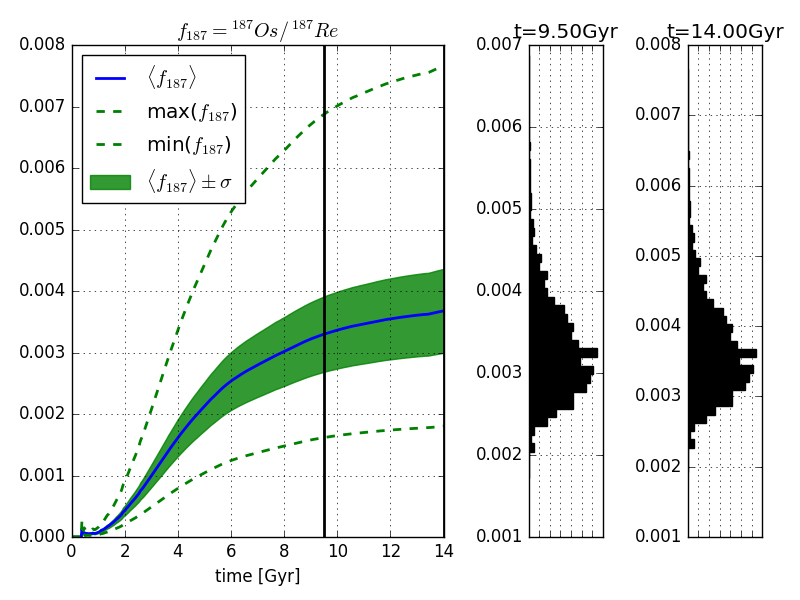
\includegraphics[width=\linewidth]{results/MCExperiment_revised_2/combined_plot_div.png}
    \caption{\label{fig:MCExperiment-nodecay-div}
      Fraction of \os{187} to \re{187} in the interstellar medium of the galaxy modelled by \omegamodel.
    }
  \end{subfigure}
  \caption[\expone before \betadecay]{\label{fig:MCExperiment-nodecay}
    The mass and mass fractions in the interstellar medium \textit{before} \betadecay is applied. Only nucleosynthesis/production from stellar sources is considered.

    The far left plot of all subfigures represent the timeevolution of the mass/mass-fraction in the interstellar medium, while the two right plots represent the uncertainty distribution at a given point in time. The points in time are 9.5 Gyrs (the formation of the solar system) and 14 Gyrs (current time). The points in time are also shown by black vertical lines in the far left plot.
  }
\end{figure}

%add plots of Os-187, Re-187, Os-187/Re-187 for regular MCExperiment
\begin{figure}
  \centering
  \begin{subfigure}{\subfigwidth}
    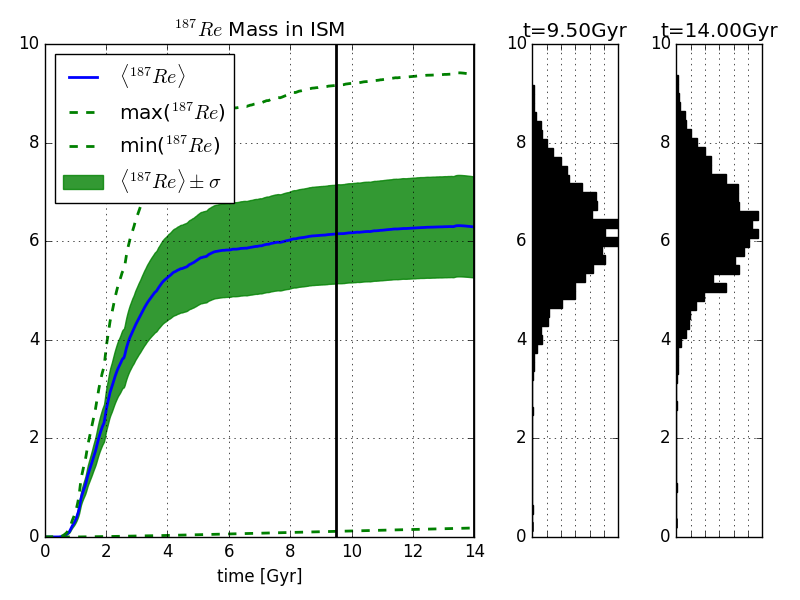
\includegraphics[width=\linewidth]{results/MCExperiment_revised_2/combined_plot_Re-187_decayed.png}
    \caption{\label{fig:MCExperiment-re187}
      Total mass of \re{187} in the interstellar medium of the galaxy modelled by \omegamodel.
    }
  \end{subfigure}
  \begin{subfigure}{\subfigwidth}
    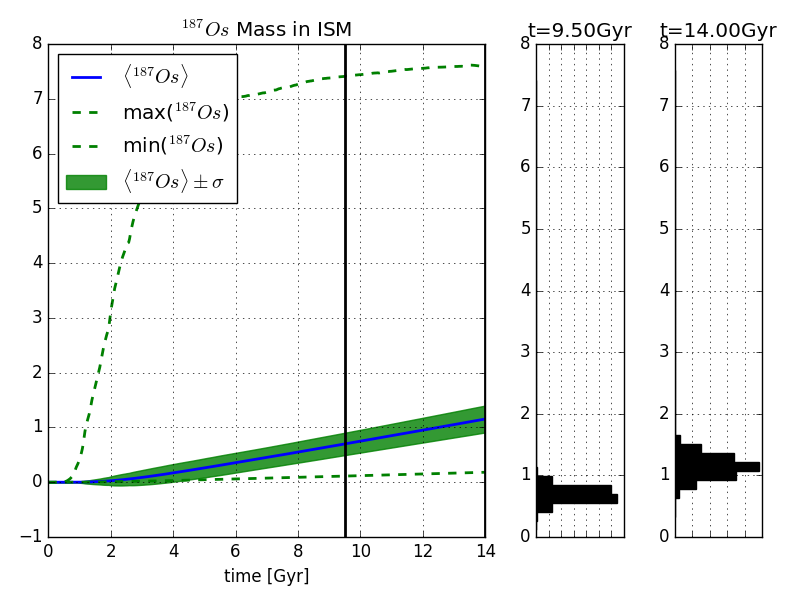
\includegraphics[width=\linewidth]{results/MCExperiment_revised_2/combined_plot_Os-187_decayed.png}
    \caption{\label{fig:MCExperiment-os187}
      Total mass of \os{187} in the interstellar medium of the galaxy modelled by \omegamodel.
  }
  \end{subfigure}
  \begin{subfigure}{\subfigwidth}
    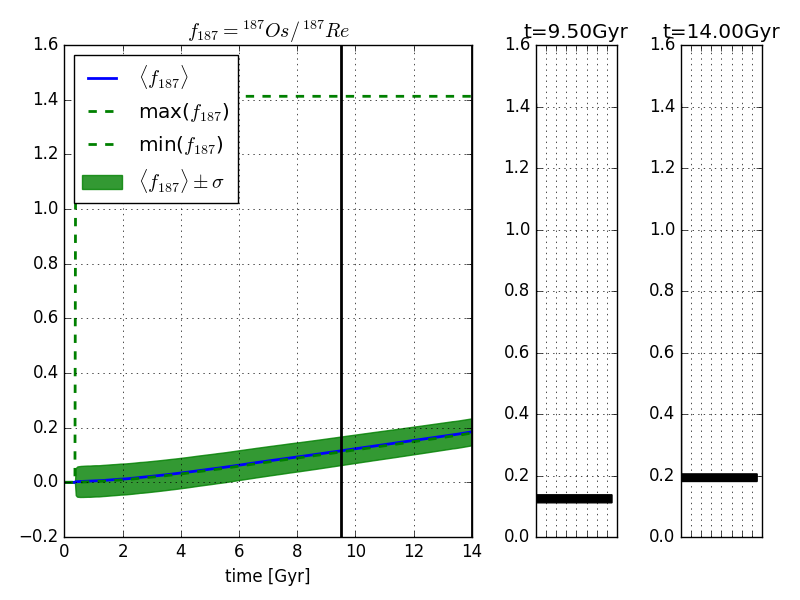
\includegraphics[width=\linewidth]{results/MCExperiment_revised_2/combined_plot_div_decayed.png}
    \caption{\label{fig:MCExperiment-div}
      Fraction of \os{187} to \re{187} in the interstellar medium of the galaxy modelled by \omegamodel.
    }
  \end{subfigure}
  \caption[\expone after \betadecay]{\label{fig:MCExperiment}
    The mass and mass fractions in the interstellar medium \textit{after} \betadecay is applied. Nucleosynthesis/production from stellar sources is considered as well as the radioactive decay from \re{187} to \os{187}.

    The far left plot of all subfigures represent the timeevolution of the mass/mass-fraction in the interstellar medium, while the two right plots represent the uncertainty distribution at a given point in time. The points in time are 9.5 Gyrs (the formation of the solar system) and 14 Gyrs (current time). The points in time are also shown by black vertical lines in the far left plot.
  }
\end{figure}

%add plots of Os-187, Re-187, Os-187/Re-187 for MCExperiment w/IMFslope
\begin{figure}
  \centering
  \begin{subfigure}{\subfigwidth}
    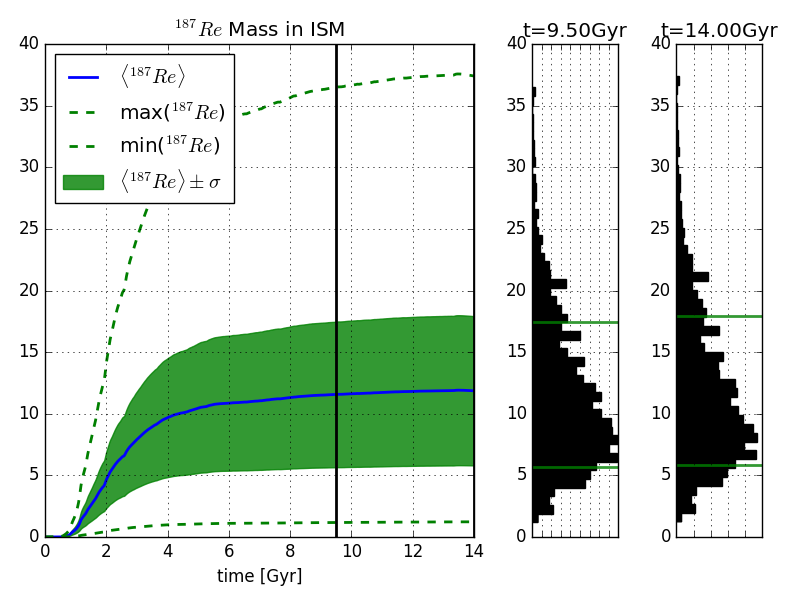
\includegraphics[width=\linewidth]{results/MCExperiment_revised_2_imfslope/combined_plot_Re-187_decayed.png}
    \caption{\label{fig:MCExperiment-imfslope-re187}
      Mass of \re{187} in the interstellar medium of the galaxy modelled by \omegamodel.
    }
  \end{subfigure}
  \begin{subfigure}{\subfigwidth}
    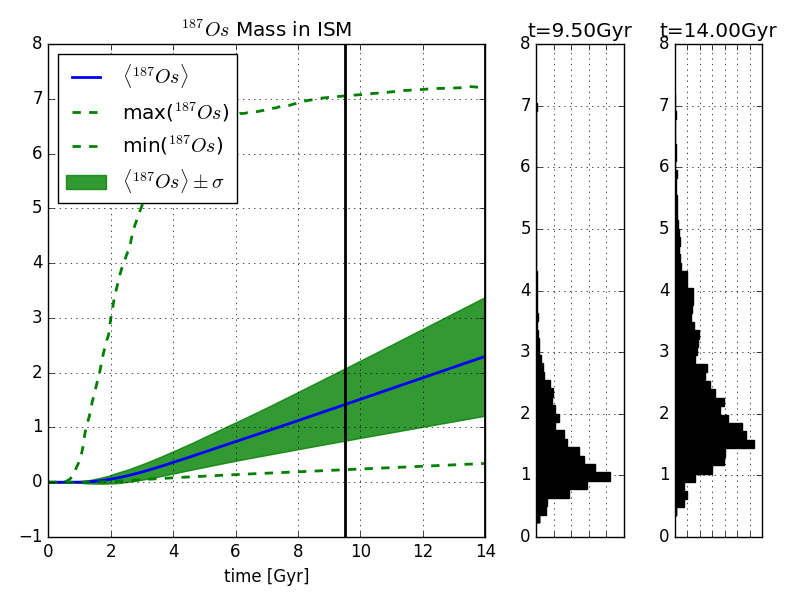
\includegraphics[width=\linewidth]{results/MCExperiment_revised_2_imfslope/combined_plot_Os-187_decayed.png}
    \caption{\label{fig:MCExperiment-imfslope-os187}
      Mass of \re{187} in the interstellar medium of the galaxy modelled by \omegamodel.
    }
  \end{subfigure}
  \begin{subfigure}{\subfigwidth}
    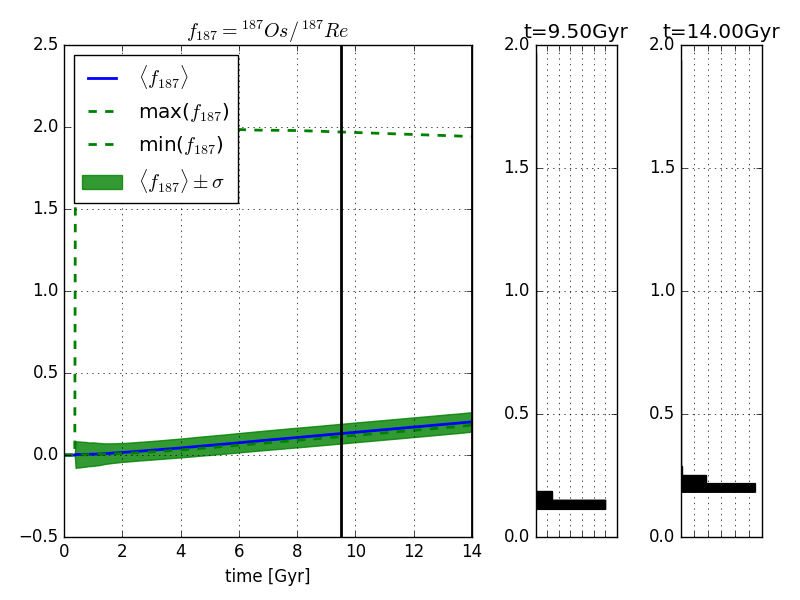
\includegraphics[width=\linewidth]{results/MCExperiment_revised_2_imfslope/combined_plot_div_decayed.png}
    \caption{\label{fig:MCExperiment-imfslope-div}
      Fraction of \os{187} to \re{187} in the interstellar medium of the galaxy modelled by \omegamodel.
    }
  \end{subfigure}
  \caption[\exptwo after \betadecay]{\label{fig:MCExperiment-imfslope}
    The mass and mass fractions in the interstellar medium \textit{after} \betadecay is applied and uncertainty in the high mass slope of the initial mass function. Nucleosynthesis/production from stellar sources is considered as well as the radioactive decay from \re{187} to \os{187}. The amount of type II supernovae are also varied because the high mass slope of the initial mass function gives more massive stars, which in turn give more type II supernovae.

    The far left plot of all subfigures represent the timeevolution of the mass/mass-fraction in the interstellar medium, while the two right plots represent the uncertainty distribution at a given point in time. The points in time are 9.5 Gyrs (the formation of the solar system) and 14 Gyrs (current time). The points in time are also shown by black vertical lines in the far left plot.
  }
\end{figure}

%(add plots of Os-187, Re-187, Os-187/Re-187 for MCExperiment w/NSMparameters)

\FloatBarrier
